\XtoCBlock{Int2Real}
\label{block:Int2Real}
\begin{figure}[H]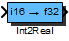
\includegraphics{Int2Real}\end{figure} 

\begin{XtoCtabular}{Inports}
In & Integer input\tabularnewline
\hline
\end{XtoCtabular}


\begin{XtoCtabular}{Outports}
Out & Real output\tabularnewline
\hline
\end{XtoCtabular}

\begin{XtoCMaskParamTabular}{Mask Parameters}
\rowcolor[gray]{0.8}\textbf{Name} & \textbf{ID} & \textbf{Description}\tabularnewline\hline
Scale & 1 & Scaling factor from integer to real\tabularnewline
\hline
\end{XtoCMaskParamTabular}

\subsubsection*{Description:}
Conversion block from integer (fixed point) datatypes to real (floating point) datatypes.

  Out = In * Scale 

% include optional documentation file
\InputIfFileExists{\XcHomePath/Library/General/Doc/Int2Real_Info.tex}{\vspace{1ex}}{}

\subsubsection*{Implementations:}
\begin{tabular}{l l}
\textbf{FiP8\_Float32} & 8 Bit Fixed Point to 32 Bit Floating Point Implementation\tabularnewline
\textbf{FiP16\_Float32} & 16 Bit Fixed Point to 32 Bit Floating Point Implementation\tabularnewline
\textbf{FiP32\_Float32} & 32 Bit Fixed Point to 32 Bit Floating Point Implementation\tabularnewline
\textbf{FiP8\_Float64} & 8 Bit Fixed Point to 64 Bit Floating Point Implementation\tabularnewline
\textbf{FiP16\_Float64} & 16 Bit Fixed Point to 64 Bit Floating Point Implementation\tabularnewline
\textbf{FiP32\_Float64} & 32 Bit Fixed Point to 64 Bit Floating Point Implementation\tabularnewline
\textbf{Bool\_Float32} & Boolean to 32 Bit Floating Point Implementation\tabularnewline
\textbf{Bool\_Float64} & Boolean to 64 Bit Floating Point Implementation\tabularnewline
\end{tabular}

\XtoCImplementation{FiP8\_Float32}
\nopagebreak[0]

8 Bit Fixed Point to 32 Bit Floating Point Implementation

\begin{XtoCtabular}{Inports Data Type}
In & int8\tabularnewline
\hline
\end{XtoCtabular}

\begin{XtoCtabular}{Outports Data Type}
Out & float32\tabularnewline
\hline
\end{XtoCtabular}

\ifdefined \AddTestReports
\InputIfFileExists{\XcHomePath/Library/General/Doc/Test-Results/Test_Int2Real_FiP8_Float32.tex}{}{}
\fi
\XtoCImplementation{FiP16\_Float32}
\nopagebreak[0]

16 Bit Fixed Point to 32 Bit Floating Point Implementation

\begin{XtoCtabular}{Inports Data Type}
In & int16\tabularnewline
\hline
\end{XtoCtabular}

\begin{XtoCtabular}{Outports Data Type}
Out & float32\tabularnewline
\hline
\end{XtoCtabular}

\ifdefined \AddTestReports
\InputIfFileExists{\XcHomePath/Library/General/Doc/Test-Results/Test_Int2Real_FiP16_Float32.tex}{}{}
\fi
\XtoCImplementation{FiP32\_Float32}
\nopagebreak[0]

32 Bit Fixed Point to 32 Bit Floating Point Implementation

\begin{XtoCtabular}{Inports Data Type}
In & int32\tabularnewline
\hline
\end{XtoCtabular}

\begin{XtoCtabular}{Outports Data Type}
Out & float32\tabularnewline
\hline
\end{XtoCtabular}

\ifdefined \AddTestReports
\InputIfFileExists{\XcHomePath/Library/General/Doc/Test-Results/Test_Int2Real_FiP32_Float32.tex}{}{}
\fi
\XtoCImplementation{FiP8\_Float64}
\nopagebreak[0]

8 Bit Fixed Point to 64 Bit Floating Point Implementation

\begin{XtoCtabular}{Inports Data Type}
In & int8\tabularnewline
\hline
\end{XtoCtabular}

\begin{XtoCtabular}{Outports Data Type}
Out & float64\tabularnewline
\hline
\end{XtoCtabular}

\ifdefined \AddTestReports
\InputIfFileExists{\XcHomePath/Library/General/Doc/Test-Results/Test_Int2Real_FiP8_Float64.tex}{}{}
\fi
\XtoCImplementation{FiP16\_Float64}
\nopagebreak[0]

16 Bit Fixed Point to 64 Bit Floating Point Implementation

\begin{XtoCtabular}{Inports Data Type}
In & int16\tabularnewline
\hline
\end{XtoCtabular}

\begin{XtoCtabular}{Outports Data Type}
Out & float64\tabularnewline
\hline
\end{XtoCtabular}

\ifdefined \AddTestReports
\InputIfFileExists{\XcHomePath/Library/General/Doc/Test-Results/Test_Int2Real_FiP16_Float64.tex}{}{}
\fi
\XtoCImplementation{FiP32\_Float64}
\nopagebreak[0]

32 Bit Fixed Point to 64 Bit Floating Point Implementation

\begin{XtoCtabular}{Inports Data Type}
In & int32\tabularnewline
\hline
\end{XtoCtabular}

\begin{XtoCtabular}{Outports Data Type}
Out & float64\tabularnewline
\hline
\end{XtoCtabular}

\ifdefined \AddTestReports
\InputIfFileExists{\XcHomePath/Library/General/Doc/Test-Results/Test_Int2Real_FiP32_Float64.tex}{}{}
\fi
\XtoCImplementation{Bool\_Float32}
\nopagebreak[0]

Boolean to 32 Bit Floating Point Implementation

\begin{XtoCtabular}{Inports Data Type}
In & bool\tabularnewline
\hline
\end{XtoCtabular}

\begin{XtoCtabular}{Outports Data Type}
Out & float32\tabularnewline
\hline
\end{XtoCtabular}

\ifdefined \AddTestReports
\InputIfFileExists{\XcHomePath/Library/General/Doc/Test-Results/Test_Int2Real_Bool_Float32.tex}{}{}
\fi
\XtoCImplementation{Bool\_Float64}
\nopagebreak[0]

Boolean to 64 Bit Floating Point Implementation

\begin{XtoCtabular}{Inports Data Type}
In & bool\tabularnewline
\hline
\end{XtoCtabular}

\begin{XtoCtabular}{Outports Data Type}
Out & float64\tabularnewline
\hline
\end{XtoCtabular}

\ifdefined \AddTestReports
\InputIfFileExists{\XcHomePath/Library/General/Doc/Test-Results/Test_Int2Real_Bool_Float64.tex}{}{}
\fi
